\cohead{\Large\textbf{Symmetrie}}
\fakesubsection{Symmetrie}
Wir unterscheiden lediglich zwei Arten von Symmetrien, Achsensymmetrie zur y-Achse sowie Punktsymmetrie zum Ursprung.
\begin{tcolorbox}\centering
	\textcolor{loestc}{Das Schaubild einer ganzrationalen Funktion ist\dots}
		
	\textcolor{loestc}{\dots achsensymmetrisch zur y-Achse, wenn alle Hochzahlen gerade oder Null sind.}
		
	\textcolor{loestc}{\dots punksymmetrisch zum Ursprung, wenn alle Hochzahlen ungerade sind.}
		
	\textcolor{loestc}{\dots weder achsensymmetrisch zur y-Achse noch punktsymmetrisch zum Ursprung, wenn die Hochzahlen eine Mischung aus geraden Hochzahlen oder Null und ungeraden Hochzahlen sind.}
\end{tcolorbox}
\begin{minipage}{\textwidth}
	\begin{minipage}{0.33\textwidth}\centering
		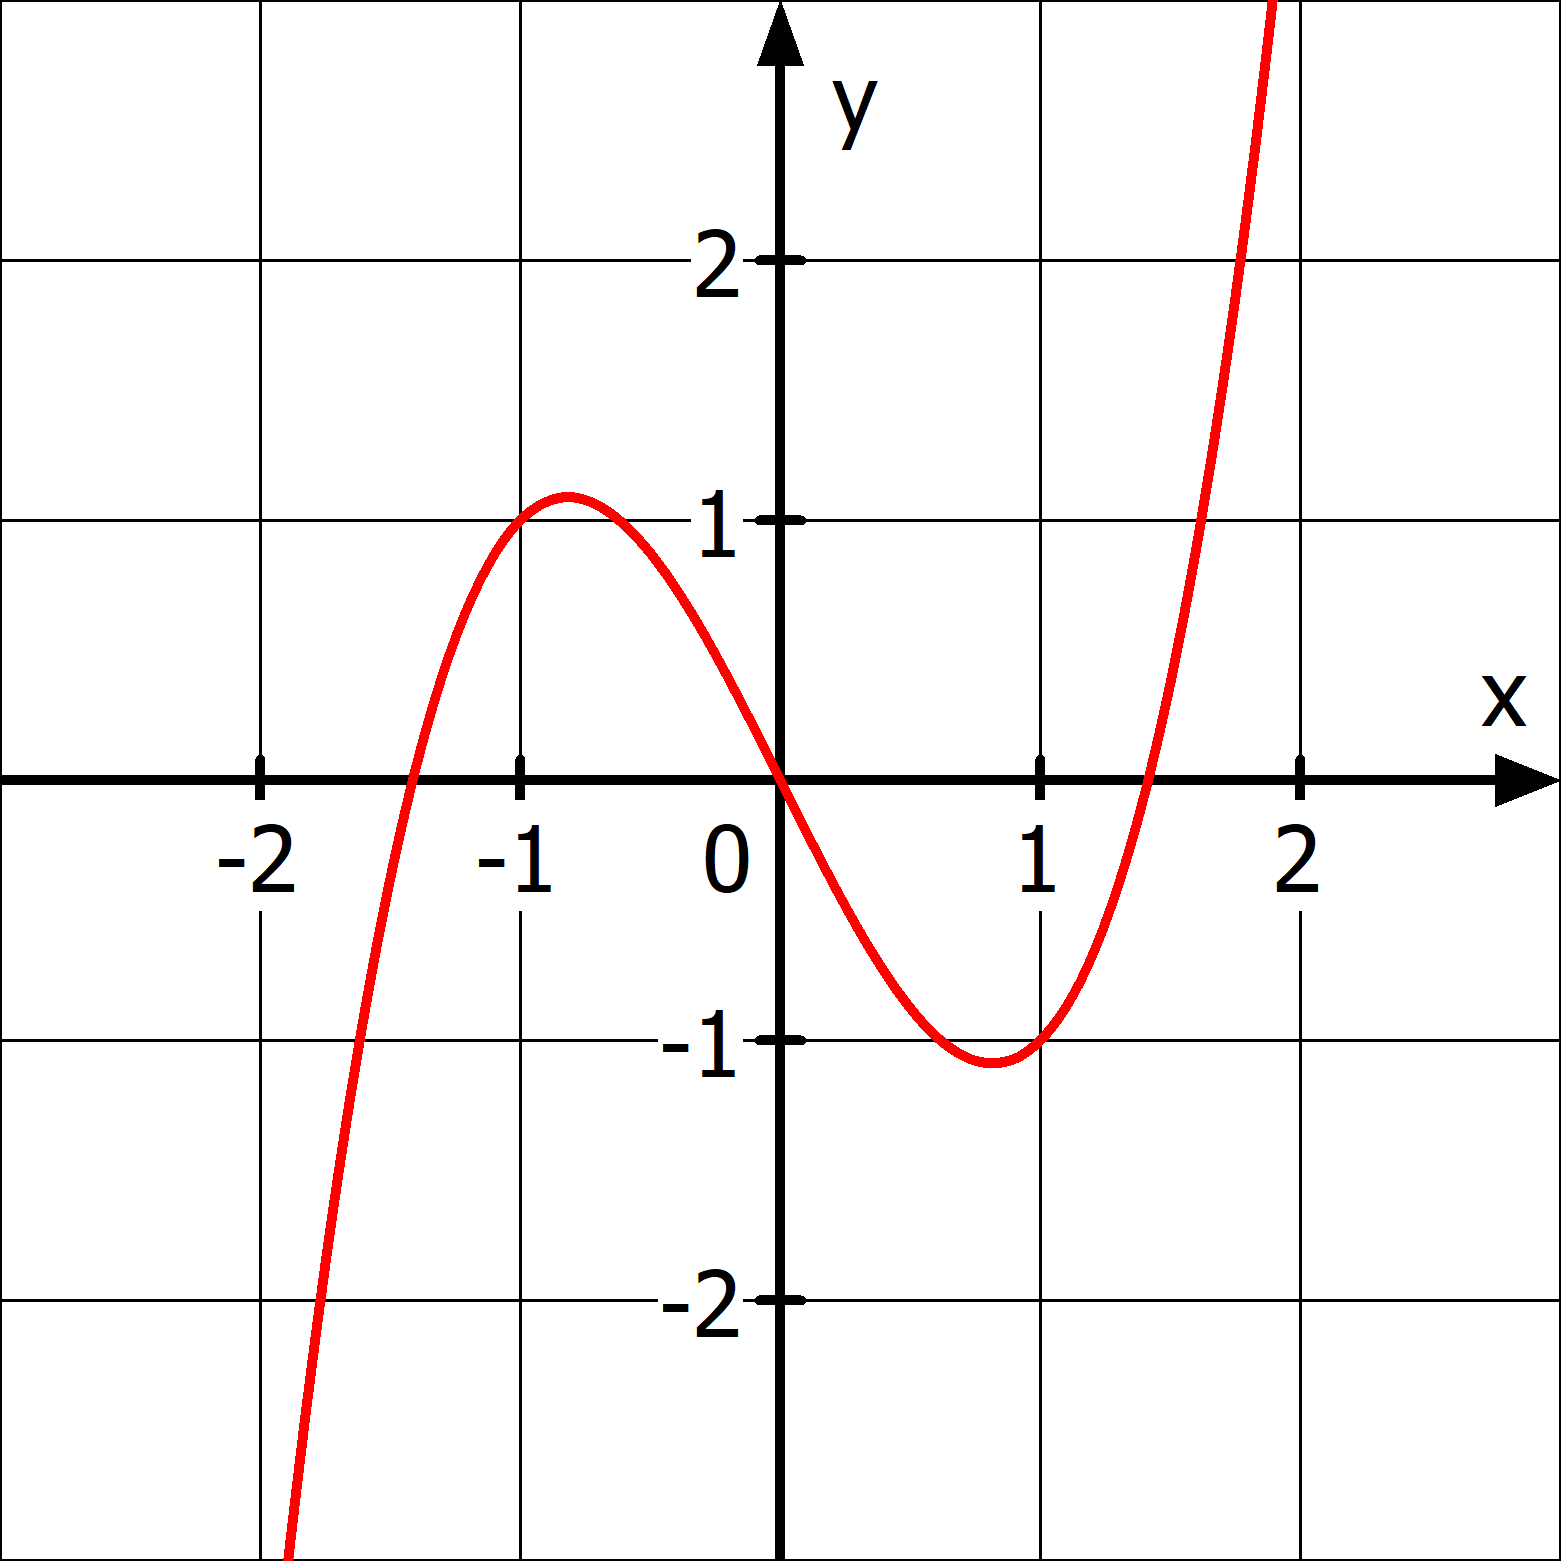
\includegraphics[width=.87\textwidth]{\ganzFkt/pics/sym4.png}
		
		\(f_1(x)=x^3-2x\)
	\end{minipage}%
	\begin{minipage}{0.33\textwidth}\centering
		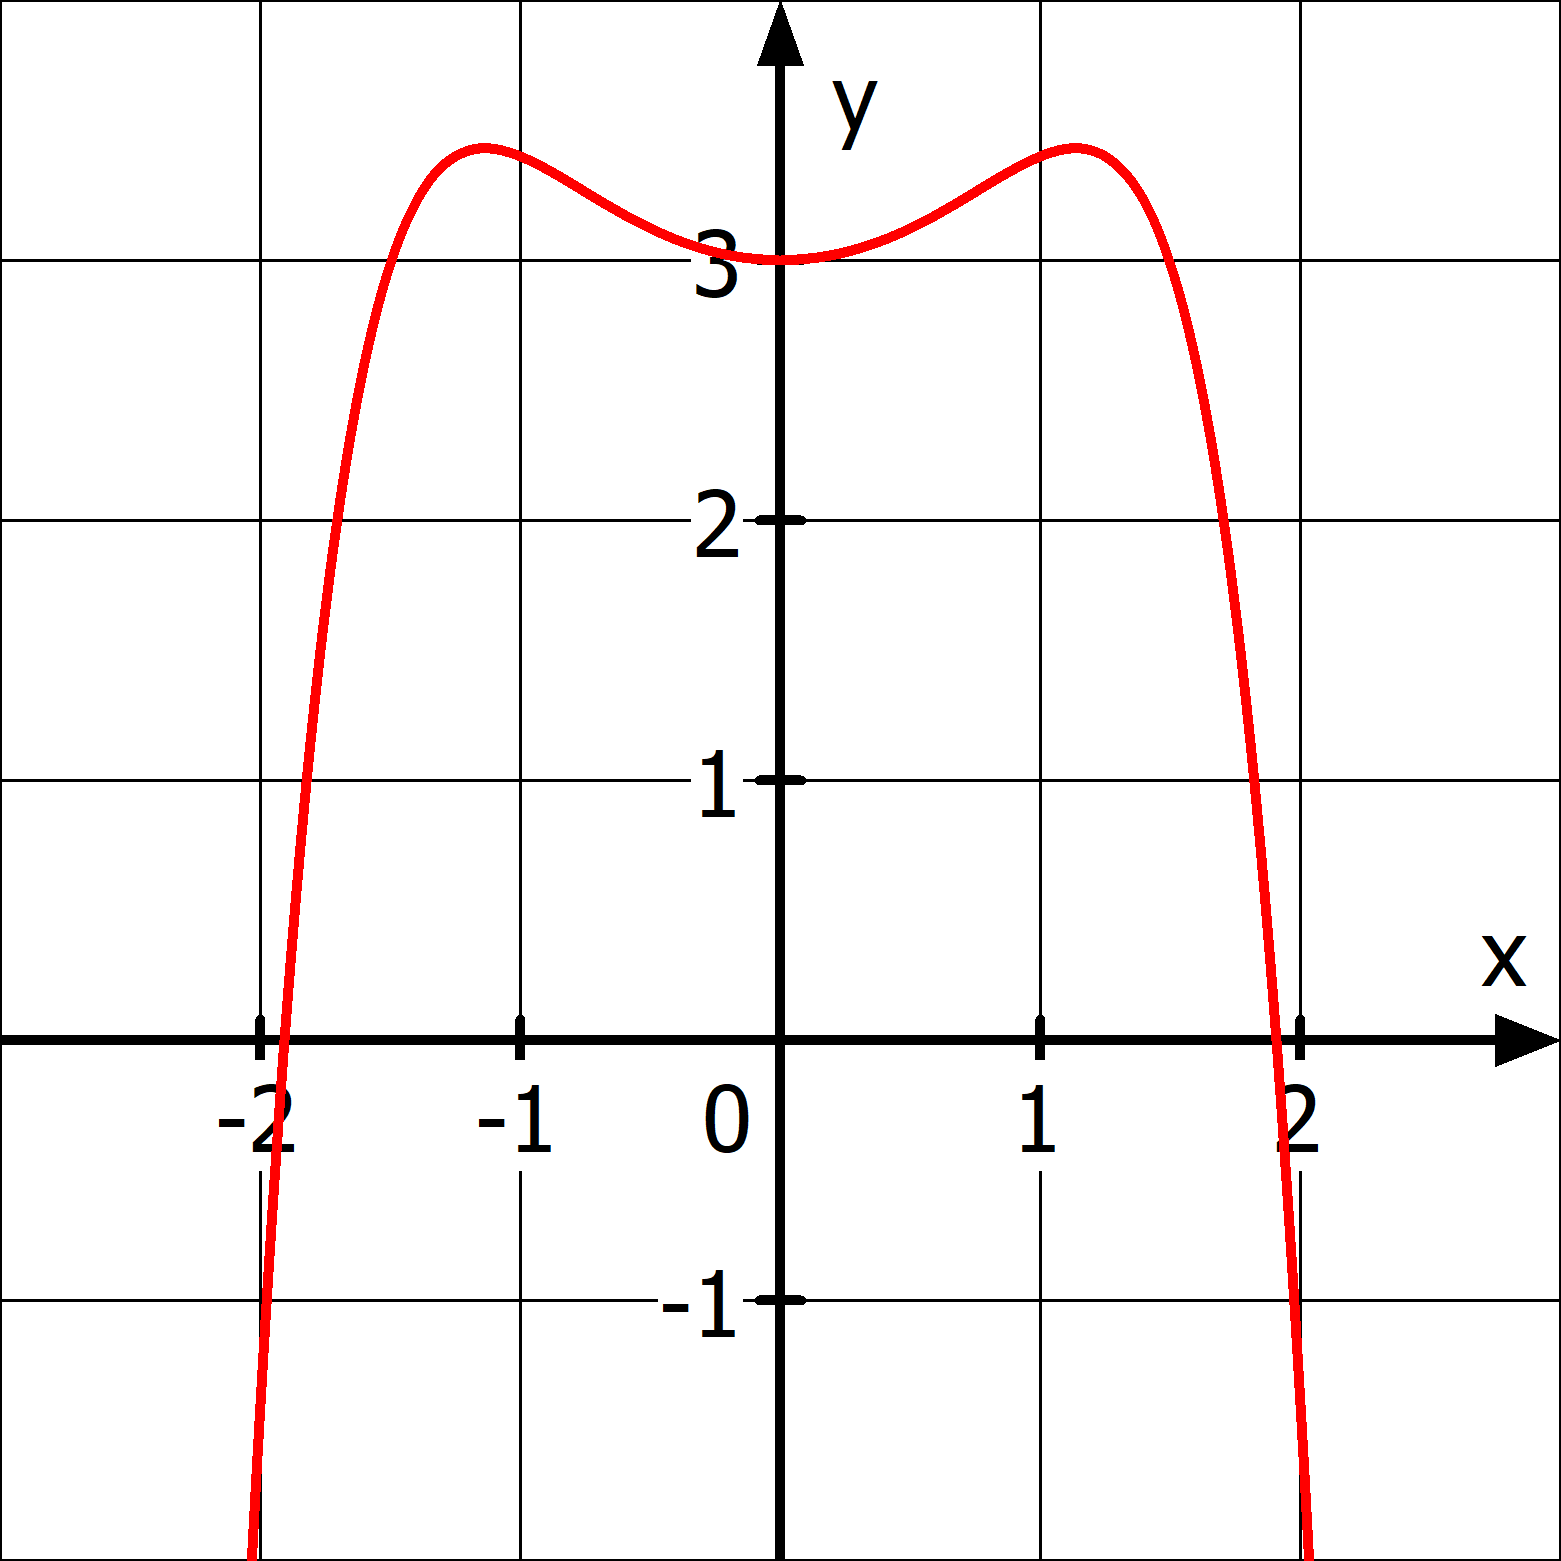
\includegraphics[width=.87\textwidth]{\ganzFkt/pics/sym2.png}
		
		\(f_2(x)=-0,1x^6+0,5x^2+3\)
	\end{minipage}%
	\begin{minipage}{0.33\textwidth}\centering
		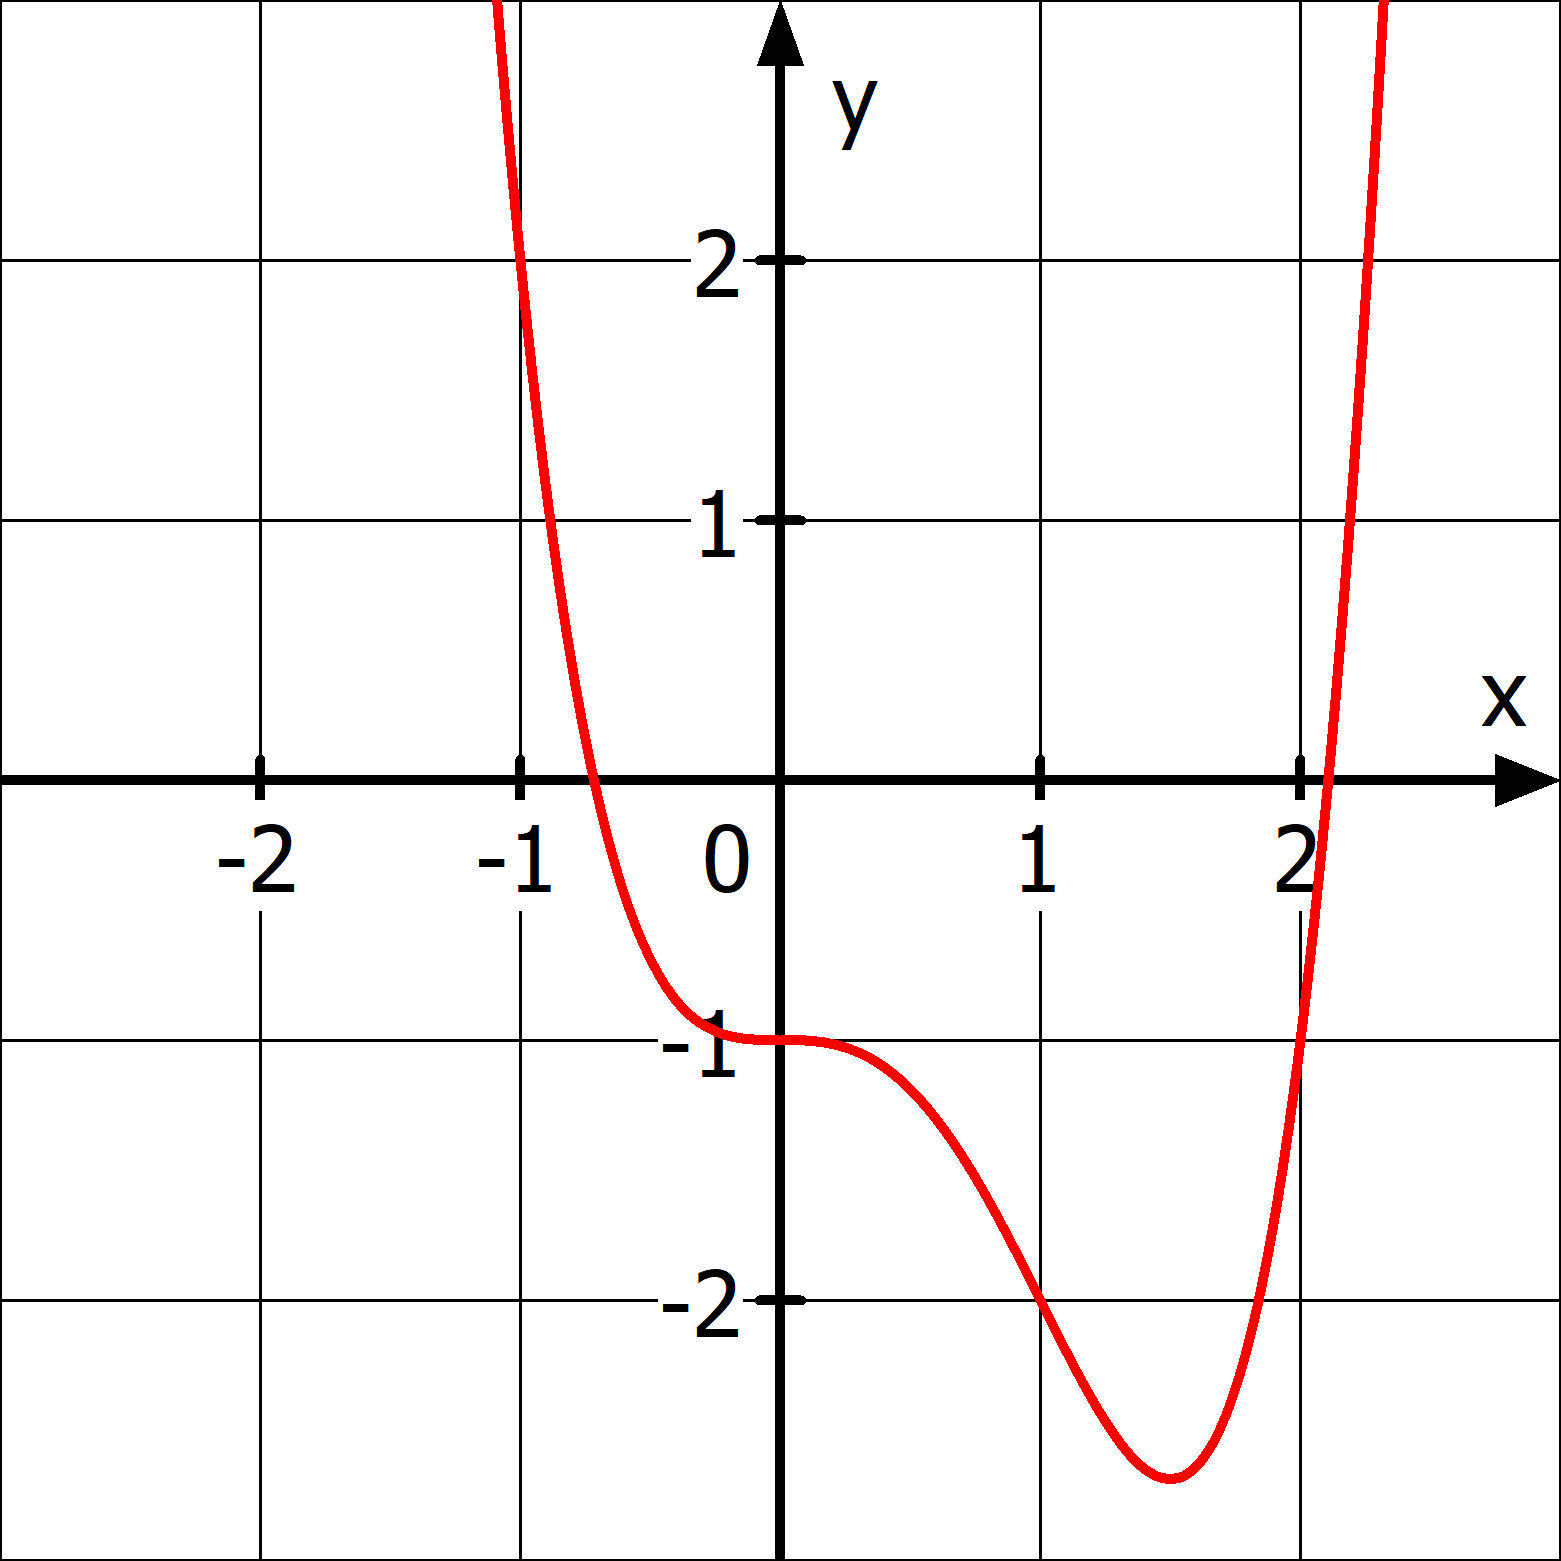
\includegraphics[width=.87\textwidth]{\ganzFkt/pics/sym8.png}
		
		\(f_3(x)=x^4-2x^3-1\)
	\end{minipage}%
	
	\medskip
	
	%%%%%%%%%%%%%%%%%%%%%%%%%%%%%%%%%%%%%%%%%%%%%%%%%%%%%%%%%%%%%%
	\begin{minipage}{0.33\textwidth}\centering
		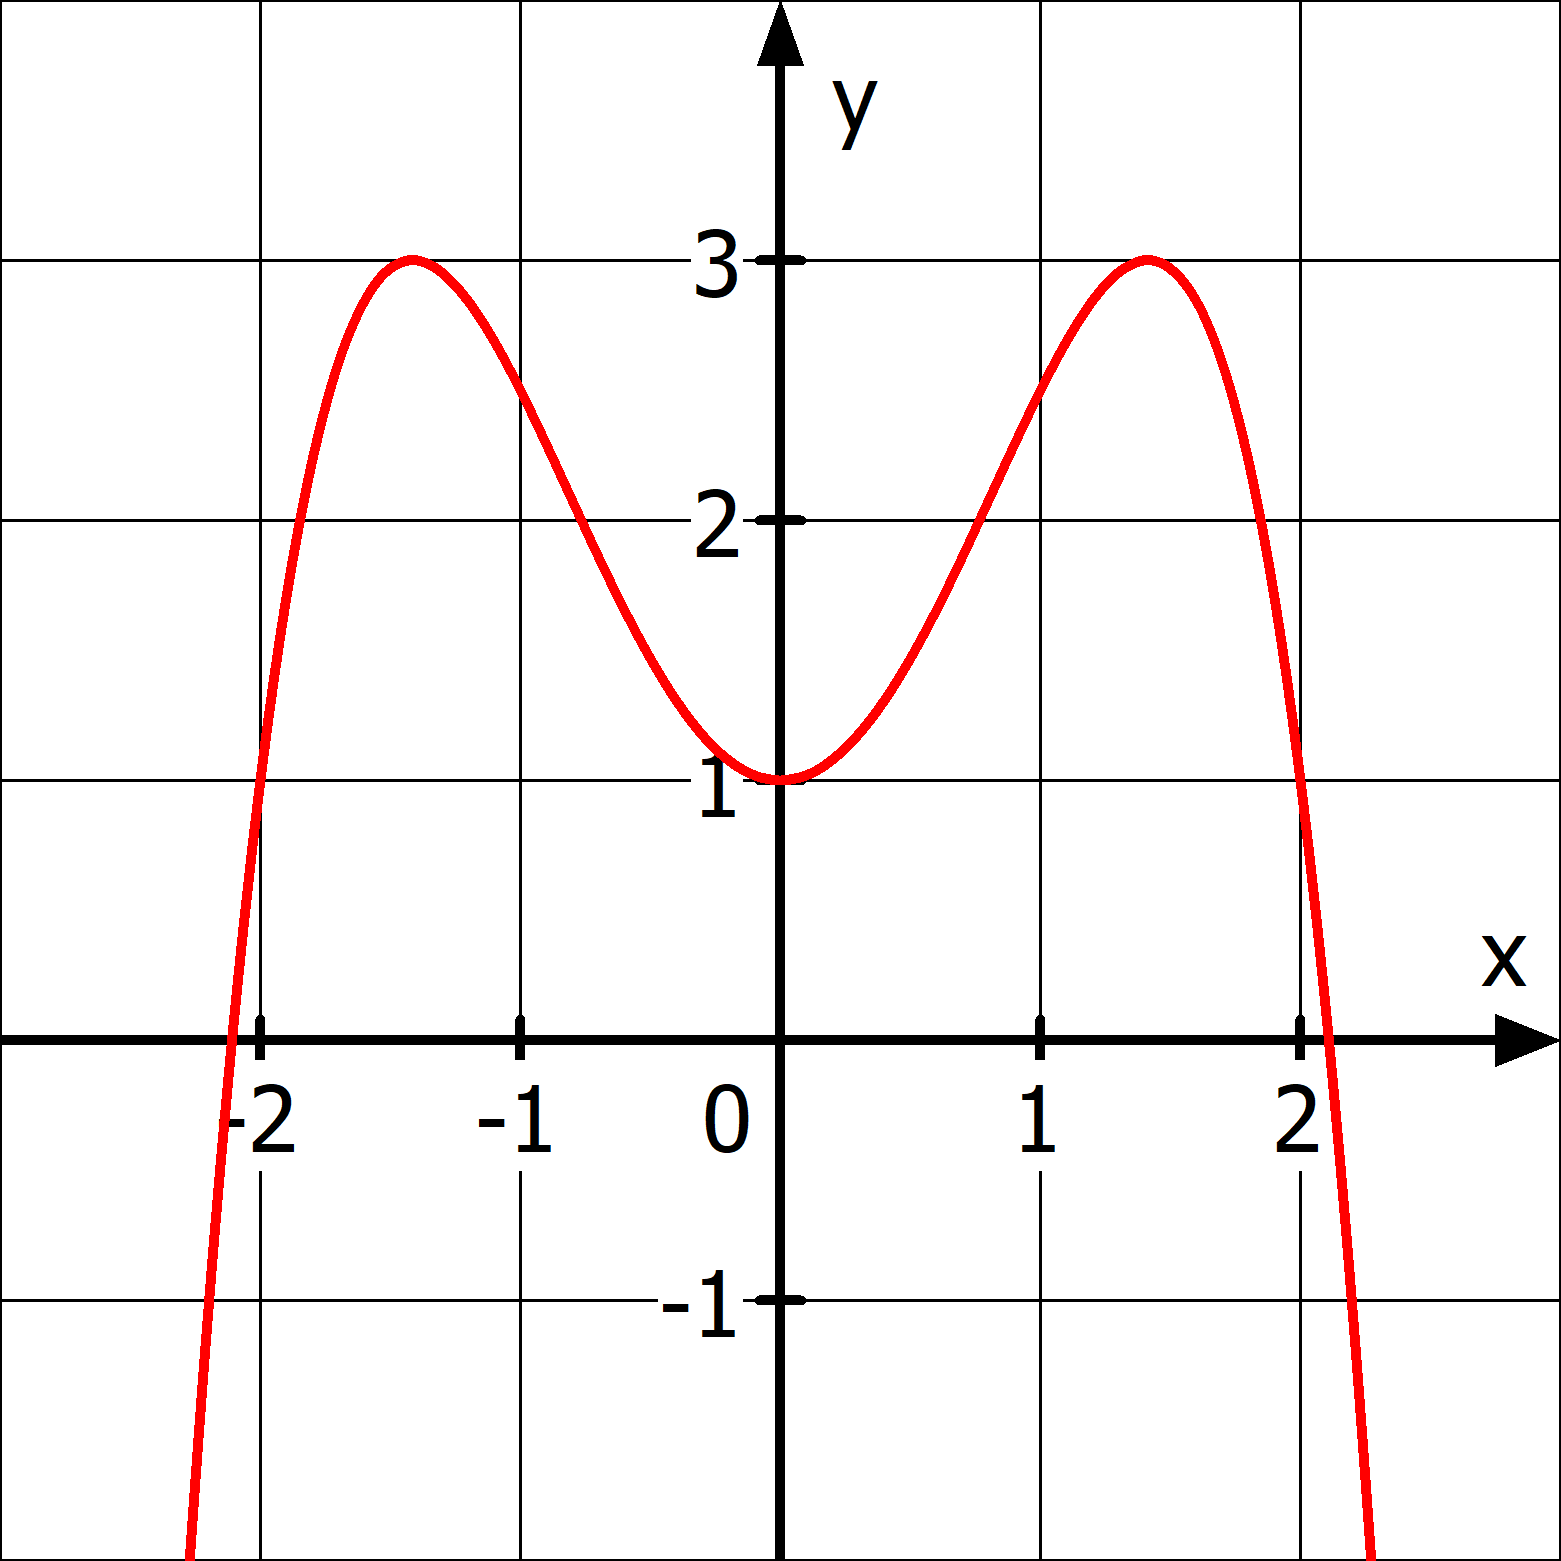
\includegraphics[width=.87\textwidth]{\ganzFkt/pics/sym1.png}
		
		\(f_4(x)= -\frac{1}{2}x^4+2x^2+1\)
	\end{minipage}%
	\begin{minipage}{0.33\textwidth}\centering
		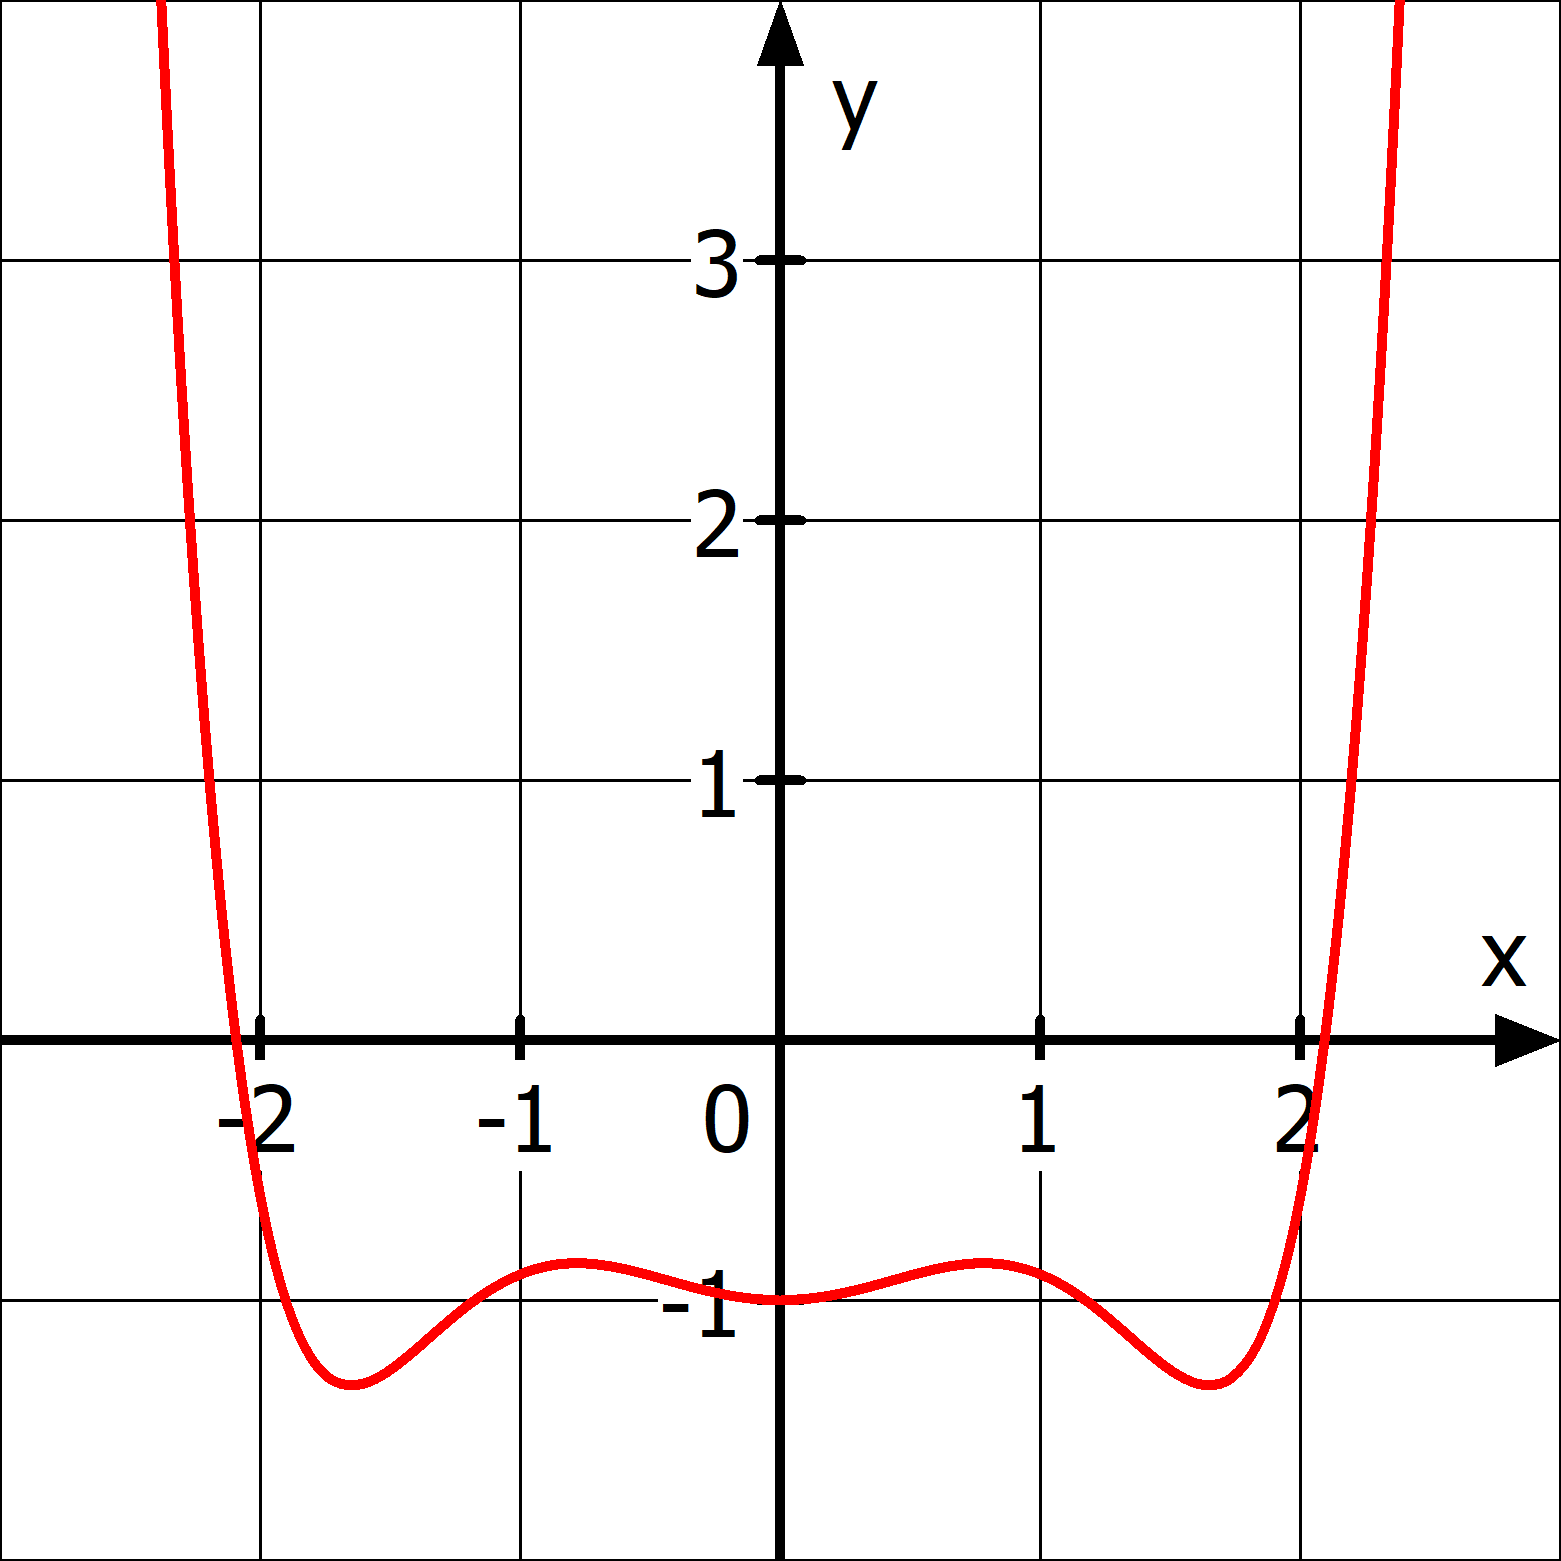
\includegraphics[width=.87\textwidth]{\ganzFkt/pics/sym3.png}
		
		\(f_5(x)=\frac{1}{10}x^6-\frac{1}{2}x^4+\frac{1}{2}x^2-1\)
	\end{minipage}%
	\begin{minipage}{0.33\textwidth}\centering
		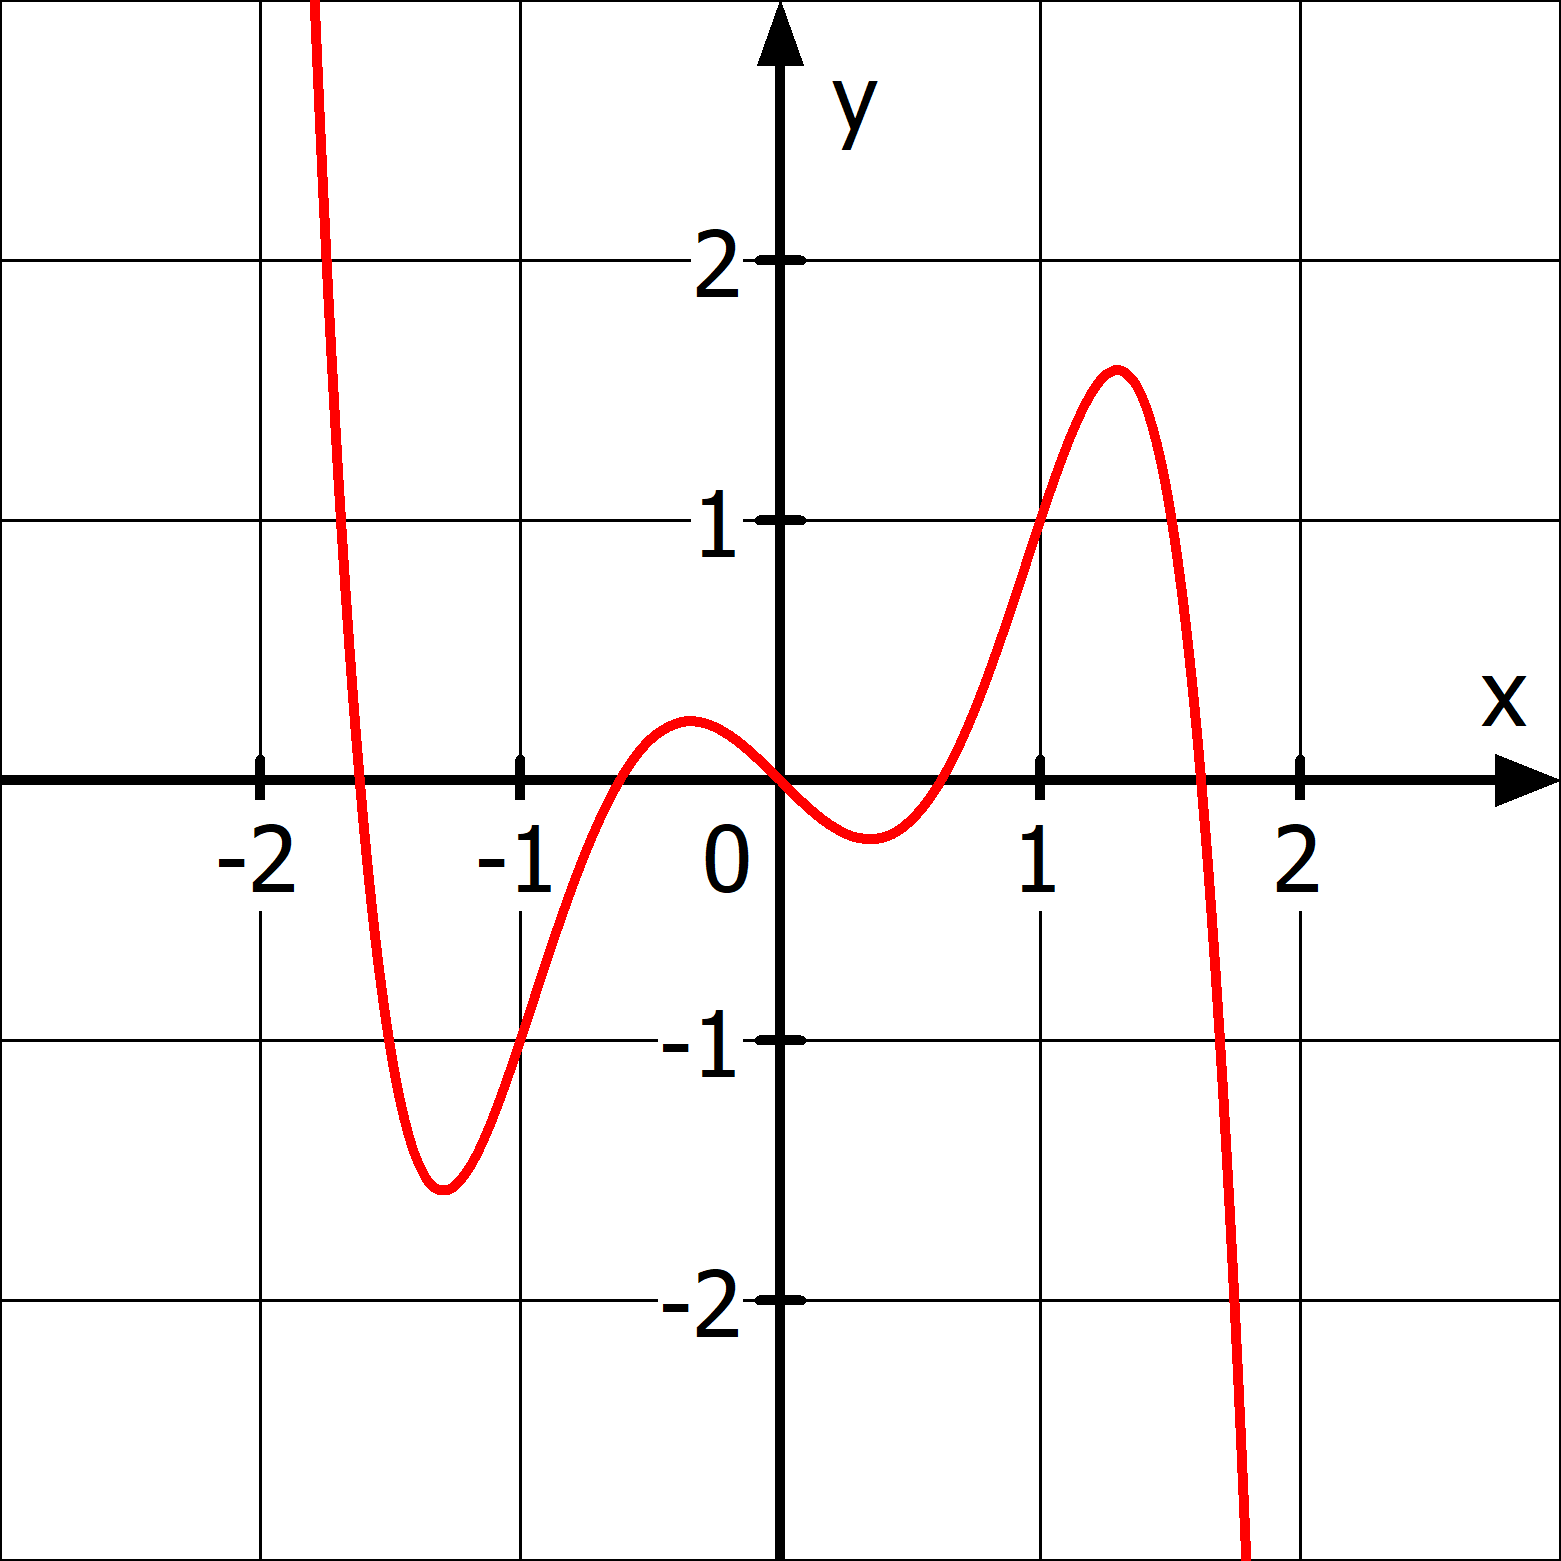
\includegraphics[width=.87\textwidth]{\ganzFkt/pics/sym5.png}
		
		\(f_6(x)=-x^5+3x^3-x\)
	\end{minipage}%
	
	\medskip
	
	%%%%%%%%%%%%%%%%%%%%%%%%%%%%%%%%%%%%%%%%%%%%
	\begin{minipage}{0.33\textwidth}\centering
		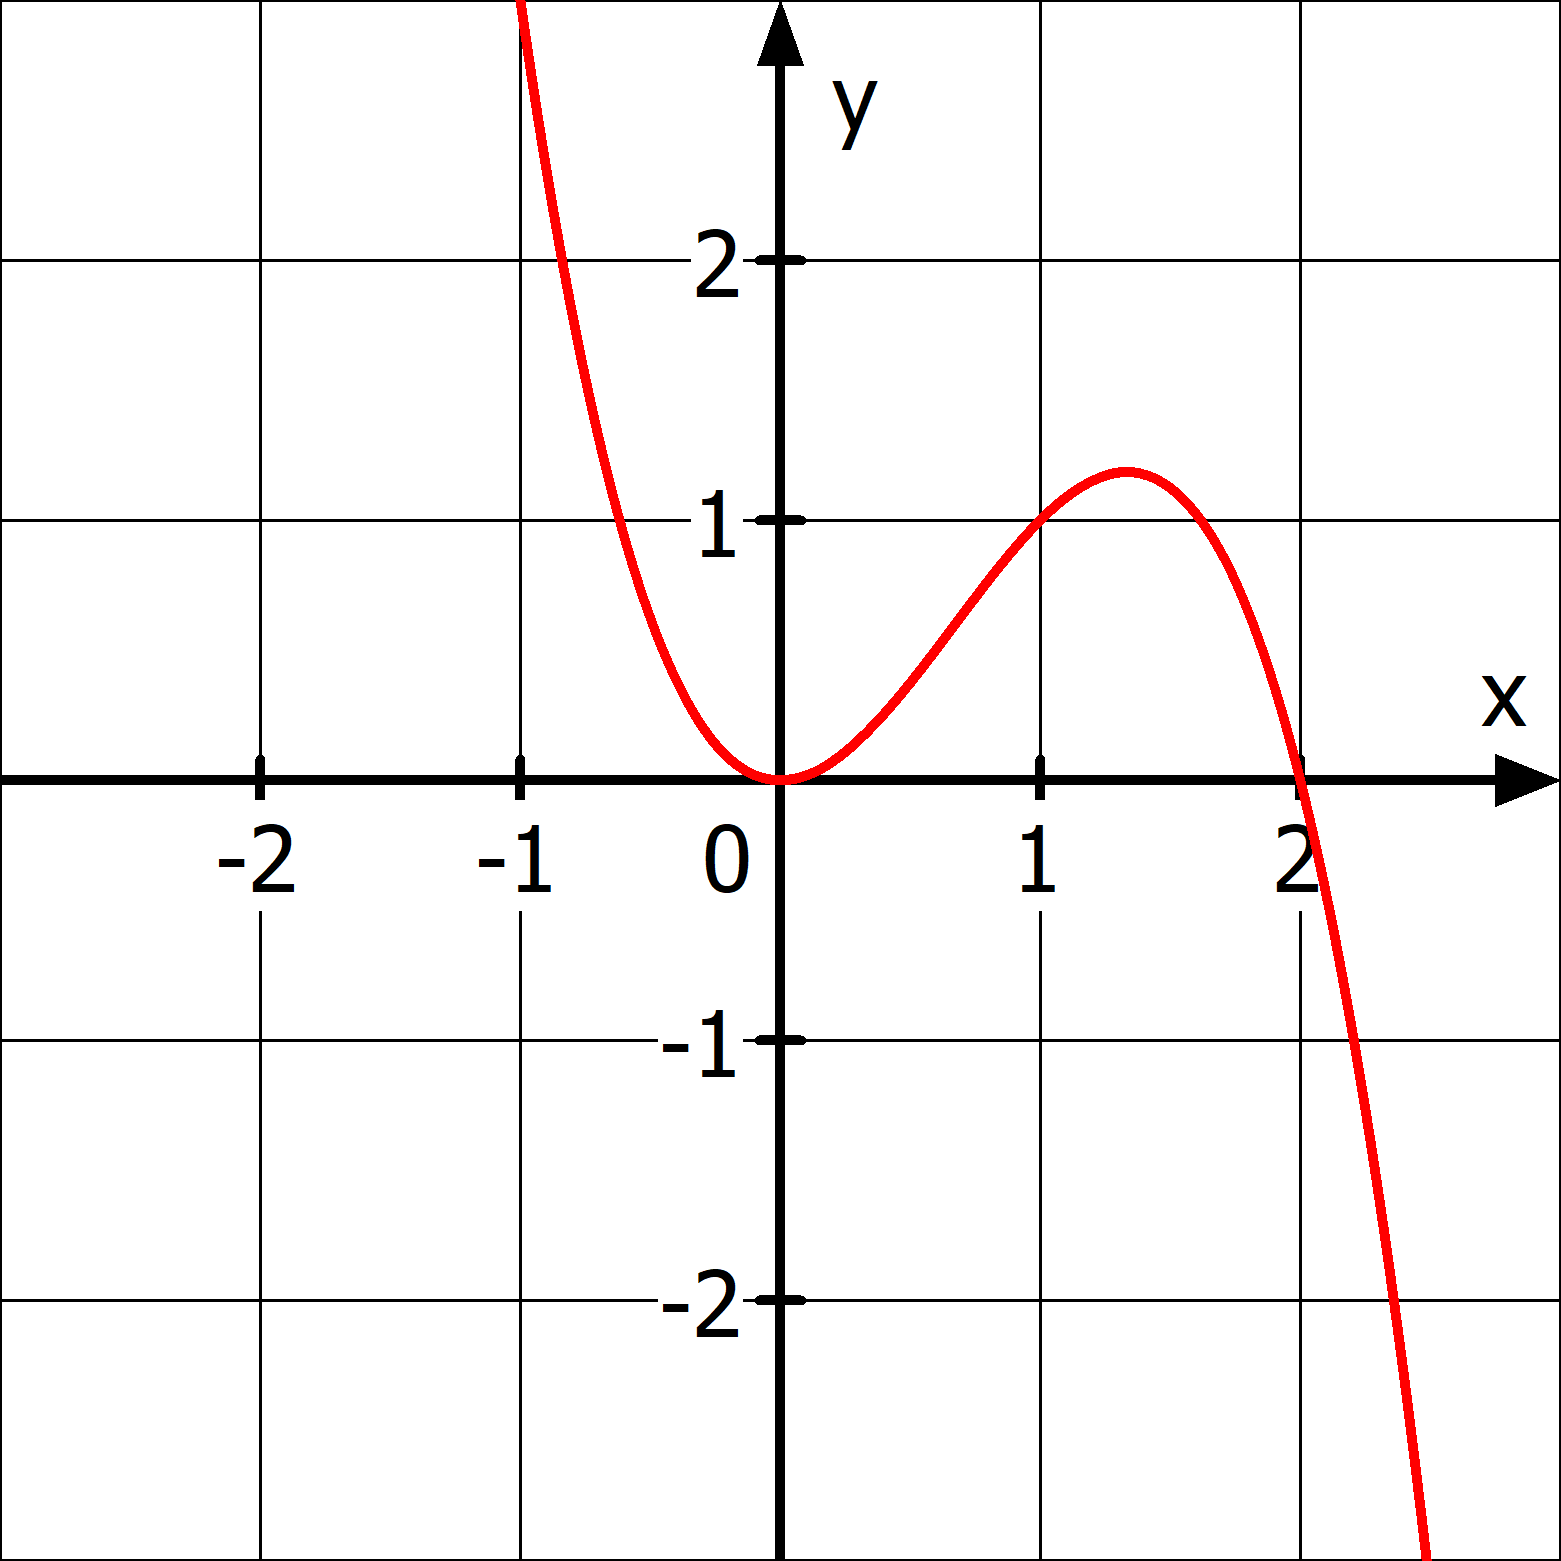
\includegraphics[width=.87\textwidth]{\ganzFkt/pics/sym7.png}
		
		\(f_7(x)=-x^3+2x^2\)
	\end{minipage}%
	\begin{minipage}{0.33\textwidth}\centering
		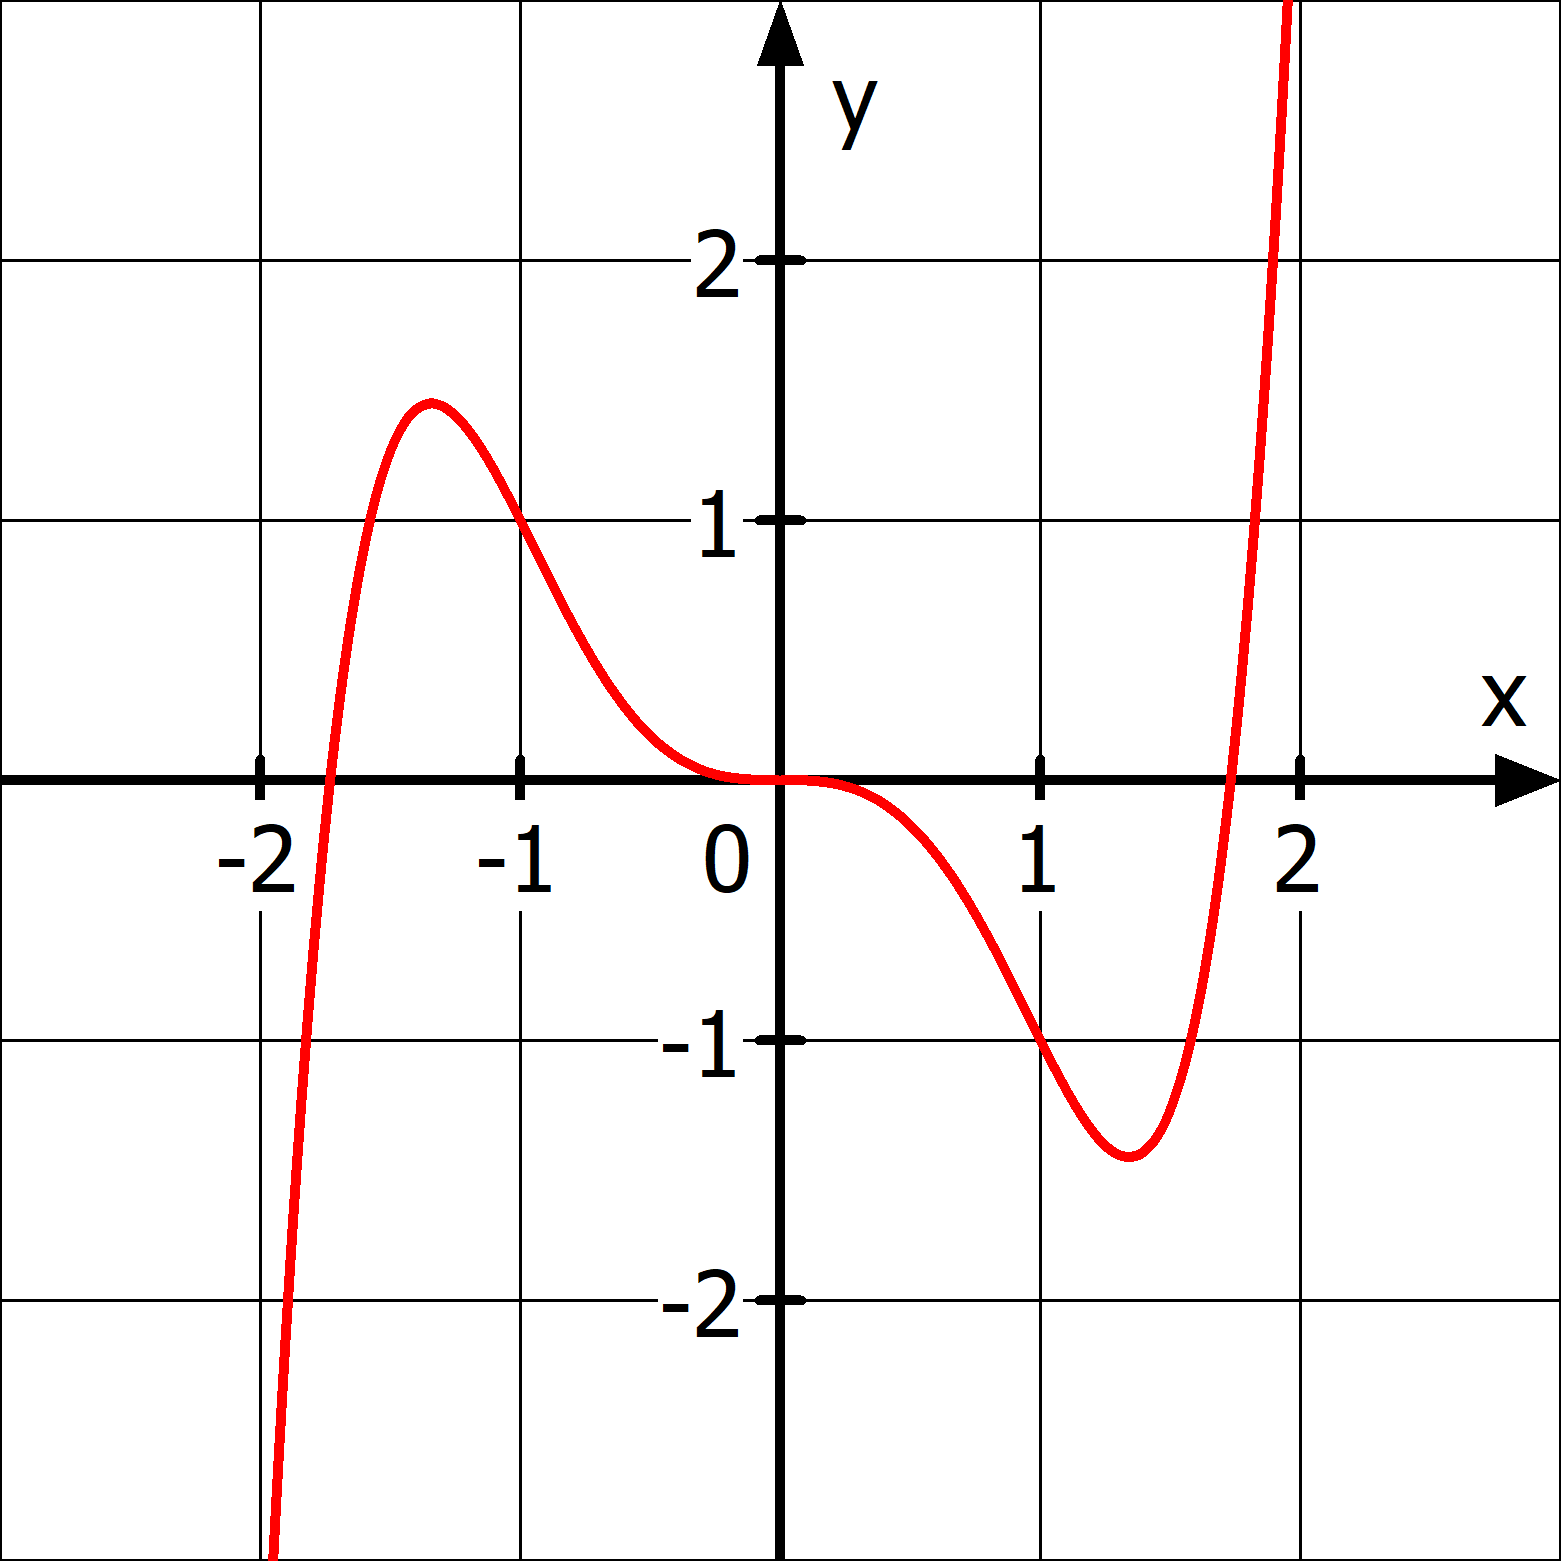
\includegraphics[width=.87\textwidth]{\ganzFkt/pics/sym6.png}
		
		\(f_8(x)=\frac{1}{2}x^5-\frac{3}{2}x^3\)
	\end{minipage}%
	\begin{minipage}{0.33\textwidth}\centering
		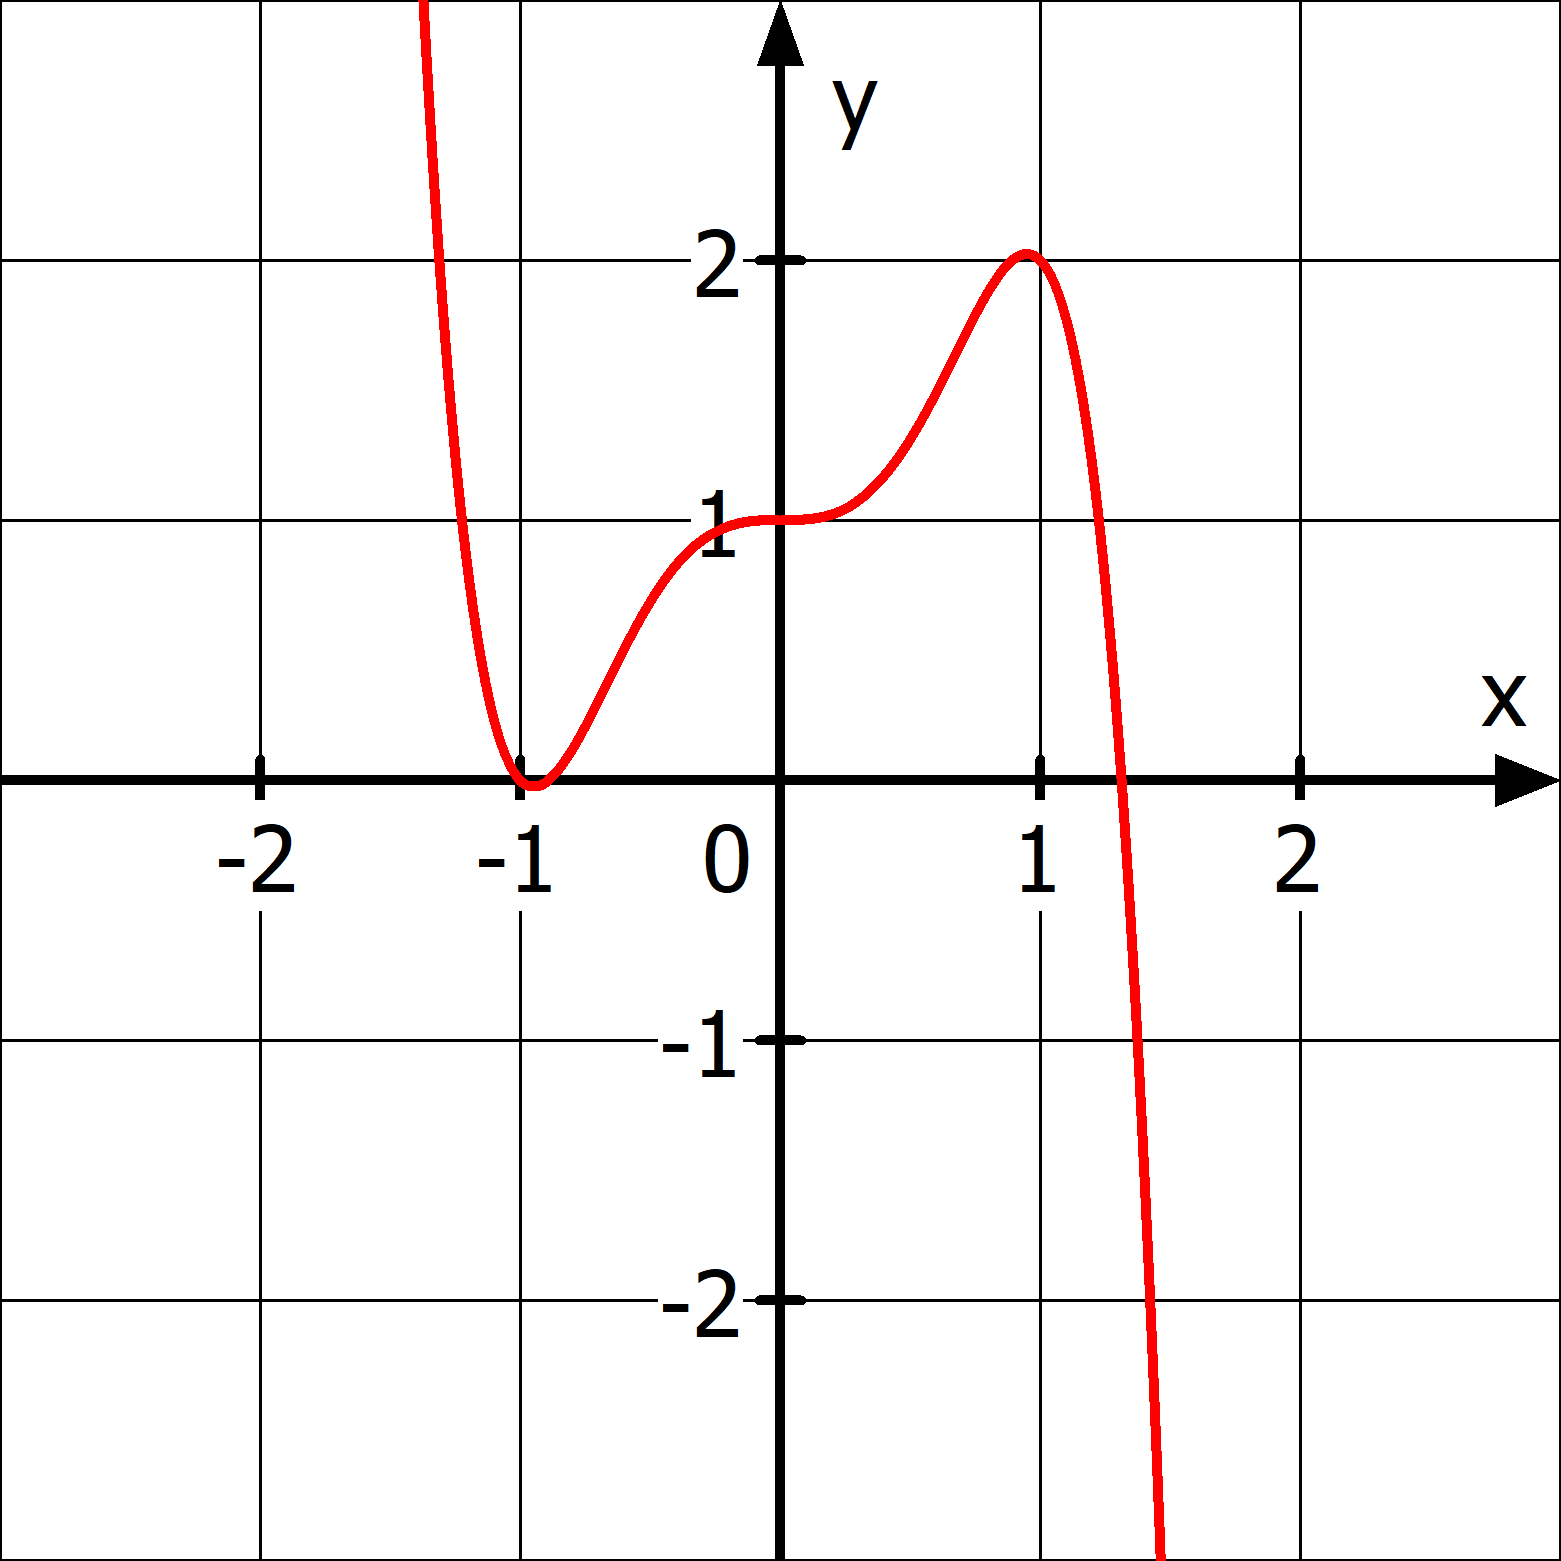
\includegraphics[width=.87\textwidth]{\ganzFkt/pics/sym9.png}
		
		\(f_9(x)=-2x^5+3x^3+1\)
	\end{minipage}%
\end{minipage}

\textcolor{loes}{Die Schaubilder von \(f_2(x),\ f_4(x)\text{ und } f_5(x)\) sind achsensymmetrisch zur y-Achse.}

\textcolor{loes}{Die Schaubilder von \(f_1(x),\ f_6(x)\text{ und } f_8(x)\) sind punktsymmetrisch zum Ursprung.}

\textcolor{loes}{Die Schaubilder von \(f_3(x),\ f_7(x)\text{ und } f_9(x)\) haben keine der beiden Symmetrien.}
\newpage
%%%%%%%%%%%%%%%%%%%%%%%%%%%%%%%%%%%%%%%%%%%%%%%%%%%%%%%%%%%%%%%%%%%%%%%%%%%%%%%%%%%%%%%%%%%%%%%%%%%%%%%%%%%%%%%%%%%%%
\begin{Exercise}[title={Untersuche auf Symmetrie}, label=ganzSymA1]
	
	\begin{minipage}{\textwidth}
		\begin{minipage}{0.49\textwidth}
			\begin{enumerate}[label=\alph*)]
				\item \(f(x)=-6x^3+2x-3\)
				\item \(g(x)=0,5x^5+x^3+2,5x\)
				\item \(h(x)=2x^6-3x^2+1\)
				\item \(i(x)=-\frac{3}{2}x^5-8x^4+x^2-1\)
			\end{enumerate}
		\end{minipage}
		\begin{minipage}{0.49\textwidth}
			\begin{enumerate}[label=\alph*)]
				\setcounter{enumi}{4}
				\item \(j(x)=-0,3x^6-12x^4-x^2-3,1\)
				\item \(k(x)=-\frac{3}{5}x^7+\frac{2}{7}x^5-\frac{11}{6}x^3-\frac{12}{5}x\)
				\item \(l(x)=-2x^3\left(x^2-2x+5\right)\)
				\item \(m(x)=3x\left(x-3\right)^2+18x^2\)
			\end{enumerate}
		\end{minipage}
	\end{minipage}
\end{Exercise}
\newpage
%%%%%%%%%%%%%%%%%%%%%%%%%%%%%%%%%%%%%%%%%
\begin{Answer}[ref=ganzSymA1]
	
	\begin{minipage}{\textwidth}
		\begin{minipage}[t]{0.5\textwidth}
			\begin{enumerate}[label=\alph*)]
				\item Hochzahlen: \(3,\ 1,\ 0\)
				
				Keine der beiden Symmetrien.
				\item Hochzahlen: \(5,\ 3,\ 1\)
				
				Punktsymmetrie zum Ursprung.
				\item Hochzahlen: \(6,\ 2,\ 0\)
				
				Achsensymmetrie zur y-Achse
				\item Hochzahlen: \(5,\ 4,\ 2,\ 0\)
				
				Keine der beiden Symmetrien.
			\end{enumerate}
		\end{minipage}%
		\begin{minipage}[t]{0.5\textwidth}
			\begin{enumerate}[label=\alph*)]
				\setcounter{enumi}{4}
				\item Hochzahlen: \(6,\ 4,\ 2,\ 0\)
				
				Achsensymmetrie zur y-Achse
				\item Hochzahlen: \(7,\ 5,\ 3,\ 1\)
				
				Punktsymmetrie zum Ursprung.
				\item \(l(x)=-2x^3\left(x^2-2x+5\right)\)
				
				\(\phantom{l(x)}=-2x^5+4x^4-10x^3\)
				
				Hochzahlen: \(5,\ 4,\ 3\)
				
				Keine der beiden Symmetrien.
				\item \(m(x)=3x\left(x-3\right)^2+18x^2=3x^3+27x\)
				
				Hochzahlen: \(3,\ 1\)
				
				Punktsymmetrie zum Ursprung.
			\end{enumerate}
		\end{minipage}%
	\end{minipage}
\end{Answer}